\chapter{Core Language Syntax and Types}\label{chp:qub-language}
In this chapter we give the formal description of the language syntax and types. We explain what
it means for a type assignment to exist as binary trees. We then show how we generalize the tree
into a sharing graph and represent it as a collection of three tuple sets in order to simplify our type inference algorithm.

\begin{figure}[h]
  \begin{framed}
    \begin{flalign*}
                         t, u, \upsilon, \phi         &\in \text{Type Variables}\\
                                      P, Q            &\in \text{Finite Predicate Set}\\
      \text{Types}\ \ \               \tau            &::= t \mid \tau \rightarrow \tau\
                                \text{where}\ \{\overset{!}{\sepimp}, \sepimp, \overset{!}{\shimp}, \shimp \} \subseteq \rightarrow \\
      \text{Predicates}\ \ \        \pi,\omega        &::= \texttt{Un}\ \tau \mid \texttt{SeFun}\ \tau \mid \texttt{ShFun}\ \tau \mid \tau \geq \tau' \\
      \text{Qualified Types}\ \ \     \rho            &::= \tau \mid \pi => \rho \\
      \text{Type schemes}\ \ \        \sigma          &::= \rho \mid \forall t. \sigma 
    \end{flalign*}
  \end{framed}
  \caption{Types \qub{}}
  \label{fig:qub-types}
\end{figure}
% Describe types
The type language consists of type variables and four binary type constructors the
sharing arrow ($\shimp$) and the separating arrow ($\sepimp$) and unrestricted
version of both the type constructors ($\overset{!}{\sepimp}, \overset{!}{\shimp}$). The sharing arrow
would mean that the function shares resources with its argument and the separating
arrow would mean that the function does not share resources with its arguments.
We would write both the arrows in an infix notation.

% Describe Predicates
The predicate system enhances the expressivity of the type system. Following the same route taken
in Quill \citep{morris_best_2016} we use the predicate $\Un{\tau}$ to denote
that the type $\tau$ is unrestricted. Unrestricted types are the ones that do not have any resources or whose resources can
be duplicated or deleted easily. Built-in lightweight types such as \HaskellF{Int}, \HaskellF{Char} are considered unrestricted types.
We write $\ShFun{\phi}$ to describe that type $\phi$ may share resources with its
argument types and  $\SeFun{\phi}$ to describe that type $\phi$ does not share any resources from its argument types.
Notice that function types can also be unrestricted i.e.e it does not have any resources. If a type $\tau$ is unrestricted i.e. it qualifies with predicate
\texttt{Un} and it also qualifies one of the function predicates---\texttt{SeFun} or \texttt{ShFun}---we write
them as $\overset{!}{\sepimp}$ and $\xrightarrow{!}$ respectively.
We also define an ordering on types by using the predicate $\geq$. The predicate $\tau \geq \tau'$ holds if the type $\tau'$
is less restricting than $\tau$ or to say $\tau$ has admits more structural rules than $\tau'$ as previously explained in \cref{sec:quill}.
The predicate entailment relations $P => Q$ are given in \cref{fig:entailment-rules}.

To keep the current system simple we have not included kinds. They are added into this system as a language extension
to enable users to define custom types using type constructors. We describe this extension in \cref{chp:datatypes}.

\begin{figure}[h]\centering
  \begin{framed}
    \begin{minipage}{0.20\linewidth}
      \begin{prooftree}
        \AxiomC{$\pi \in P$}
        \UnaryInfC{$P => \pi$}
      \end{prooftree}
    \end{minipage}%
    \begin{minipage}{0.20\linewidth}
      \begin{prooftree}
        \AxiomC{$\bigwedge_{\pi \in Q} P => \pi$}
        \UnaryInfC{$P => Q$}
      \end{prooftree}
    \end{minipage}%
    \begin{minipage}{0.20\linewidth}
      \begin{prooftree}
        \AxiomC{${\color{white}\bigwedge_{\pi \in Q}}$}
        \UnaryInfC{$P => \Un{(\tau \overset{!}{\sepimp} \tau')}$}
      \end{prooftree}
    \end{minipage}
    \begin{minipage}{0.20\linewidth}
      \begin{prooftree}
        \AxiomC{${\color{white}\bigwedge_{\pi \in Q}}$}
        \UnaryInfC{$P => \Un{(\tau \overset{!}{\sepimp} \tau')}$}
      \end{prooftree}
    \end{minipage}

    \begin{minipage}{0.20\linewidth}
      \begin{prooftree}
        \AxiomC{$\tau = \sepimp \vee \tau = \overset{!}{\sepimp}$}
        \UnaryInfC{$P => \SeFun{\tau}$}
      \end{prooftree}
    \end{minipage}%
    \begin{minipage}{0.20\linewidth}
      \begin{prooftree}
        \AxiomC{$\tau = \shimp \vee \tau = \overset{!}{\shimp}$}
        \UnaryInfC{$P => \ShFun{\tau}$}
      \end{prooftree}
    \end{minipage}%
    \begin{minipage}{0.20\linewidth}
      \begin{prooftree}
        \AxiomC{$P => \Un{\tau}$}
        \UnaryInfC{$P => \tau \geq (v \overset{!}{\sepimp} v')$}
      \end{prooftree}
    \end{minipage}%
    \begin{minipage}{0.20\linewidth}
      \begin{prooftree}
        \AxiomC{$P => \Un{\tau}$}
        \UnaryInfC{$P => \tau \geq (v \overset{!}{\shimp} v')$}
      \end{prooftree}
    \end{minipage}

    \begin{minipage}{0.30\linewidth}
      \begin{prooftree}
        \AxiomC{${\color{white}P => \tau \geq \phi t}$}
        \UnaryInfC{$P => \tau \geq (v \sepimp v')$}
      \end{prooftree}
    \end{minipage}%
    \begin{minipage}{0.30\linewidth}
      \begin{prooftree}
        \AxiomC{${\color{white}P => \tau \geq \phi t}$}
        \UnaryInfC{$P => \tau \geq (v \shimp v')$}
      \end{prooftree}
    \end{minipage}%
    \begin{minipage}{0.30\linewidth}
      \begin{prooftree}
        \AxiomC{$P => \tau \geq \phi t$}
        \AxiomC{$t\ \text{fresh}$}
        \BinaryInfC{$P => \tau \geq \phi$}
      \end{prooftree}
    \end{minipage}
  \end{framed}
  \caption{Entailment Rules}
  \label{fig:entailment-rules}
\end{figure}


% \TODO{Need some more reading/writing about multienvironment}
% Describe Type assignments
In normal type systems, the contexts are represented as sets or lists. In \BI\ they are represented as binary trees and are called bunches.
The leaf nodes contain the pair of term and its associated type. Internal nodes of the context tree are
connectives which can either be a semicolon ($;$) or a comma ($,$).
If a bunch $\Delta$ is a subtree of $\Gamma$, then we denote a subtree relation by $\Gamma(\Delta)$.
Two bunches are equivalent ($\Gamma \equiv \Delta$) if they can be transformed into another by renaming identifiers.
The bunches have a restriction that no identifier appears more than once. We restrict certain structural rules on the context
depending on the connectives being used. If contexts are combined using a comma ($,$), contraction and weakening is not admissible,
but if the contexts are combined using a semicolon ($;$) then it can undergo contraction and weakening. Exchange rule is admissible
in both the connectives. This distinction enables us to have a special treatment for resources in our language.
By associating a resource with a comma constructor, our type system will not disposed it off by using the contraction rule.
While, non-resourceful objects (or normal propositions) can be combined using the semi-colon constructor.
An example bunch is shown in \cref{fig:bunches-bi}. a and b have a shared context while c is separate from the bunch a and b.
If $\Gamma$ represents the complete bunch of \cref{fig:bunches-bi}, $\Delta \equiv (a:A; b:B)$ and $\Delta' \equiv (c:C)$
then $\Gamma \equiv \Delta,\Delta'$ and $\Gamma(\Delta)$.

\begin{figure}[h]
  \centering
  \begin{framed}
  \tikzset{every tree node/.style={minimum width=2em},
         blank/.style={draw=none},
         edge from parent/.style=
         {draw,edge from parent path={(\tikzparentnode) -- (\tikzchildnode)}},
         level distance=1.5cm}
\begin{tikzpicture}
\Tree
[.,
    [.;
        [.a:A ]
        [.b:B ]
    ]
    [.c:C ]
    ]
\end{tikzpicture}
\end{framed}
\caption{Bunches in \textbf{\em BI}}
\label{fig:bunches-bi}
\end{figure}

In our type system, we generalize the tree approach into a graph where each node represents variables or resources
and the edges between the nodes represent sharing between them. The example in \cref{fig:bunches-bi} can
be represented as what we would call a sharing graph shown in \cref{fig:sharing-graph}. A graph structure, in general,
can represent a binary tree structure and its associated operations. They represent more complex structures than
trees, thus will provide more flexibility in accepting well typed terms in our language making it more expressive.

\begin{figure}[h]
  \begin{framed}\centering
    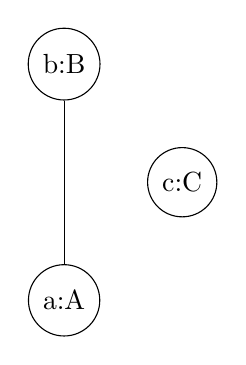
\begin{tikzpicture}
        \node[shape=circle,draw=black] (A) at (0,0) {a:A};
        \node[shape=circle,draw=black] (B) at (0,3) {b:B};
        \node[shape=circle,draw=black] (C) at (1.5,1.5) {c:C};

        \path [-] (A) edge node {} (B);
    \end{tikzpicture}
  \end{framed}
  \caption{Sharing Graph}
\label{fig:sharing-graph}
\end{figure}

We define sharing relation ($\Psi$) between variables to the collection of variables it is in sharing with.
The relation $\Psi(x, \{y_1, y_2, y_3\})$ holds if $x$ is in sharing with $\{y_1, y_2, y_3\}$.
Domain of $\Psi$ will be defined as $\texttt{dom}(\Psi) = \{x \mid (x, \vec{y}) \in \Psi \}$, where $\vec{y}$
is a shorthand for the denoting collection of variables shared with $x$. We can think of $\Psi$ to be similar to $\Gamma$,
but it contains the sharing information instead of the type of the variable. Extending the sharing for a variable will be denoted by $\Psi(x) + y$,
which would mean the variable $y$ is in sharing with $x$. We axiomatize the sharing operation to be reflexive,
symmetric and non-transitive. So to say,
\begin{flalign*}
 &\forall_{x \in \texttt{dom}(\Psi)}\ x \in \Psi(x) \tag{reflexive}\\
 &\forall_{x,y \in \texttt{dom}(\Psi)}\ \text{if}\ y \in \Psi(x)\ \text{then}\ x \in \Psi(y) \tag{symmetric}
\end{flalign*}

Our final goal is to design a simple type inferencing algorithm for a term language.
Using sharing graphs in implementing typing judgments would make the process considerably complex.
We simplify the sharing graph by flattening it into an adjacency list or a collection of 3 tuple containing the
variable identifier, its type and a collection of variables it shares with. Manipulating lists is much
easier than manipulating graphs. For example, if a resource $x$ has type $\tau$ and it shares with variables $\{y_1, y_2, y_3\}$
we would represent it as $x^{\{y_1, y_2, y_3\}}:\tau$ or just $x^{\bar{y}}:\tau$ for short.
We would write $\Gamma, x^{\vec{y}}:\tau$ to mean $\Gamma \sqcup \{x^{\vec{y}}:\tau\}$.
We can now formally define the typing context or environment as shown in \cref{fig:typing-context}.
\begin{figure}[h]
  \begin{framed}
    \begin{flalign*}
      \text{Typing Context}\ \ \      \Gamma,\Delta     &::= \epsilon \mid x^{\bar{y}}:\sigma \mid \Gamma \varoplus \Delta \mid \Gamma \circledast \Delta
  \end{flalign*}
\end{framed}
  \caption{Typing Context}
  \label{fig:typing-context}
\end{figure}

We define a few auxiliary functions on the
type assignments. \texttt{Vars}($\Gamma$) is the set of all the term variables in $\Gamma$. \texttt{Shared}($\Gamma$) computes
the set of all the term variables that are in sharing with each other. \texttt{Used}($\Gamma$) computes the
union of all the term variables in the type assignment and the term variables shared by each of those.
We define two partial operators on type assignments as shown in \cref{fig:type-assignment-operations}.
The mapping function ($\Gamma^{[\vec{a} \mapsto \vec{b}]}$) extends the sharing relation between the terms. In the sharing graph perspective
it would mean adding edges between the nodes.
\begin{figure}[h]
  \begin{framed}
    \noindent
    \begin{minipage}[h]{0.45\linewidth}
    \begin{flalign*}
      \texttt{Vars}(\Gamma, x^{\vec{y}}:\tau) &= \texttt{Vars}(\Gamma) \cup \{ x \}\\
      \texttt{Shared}(\Gamma, x^{\vec{y}}:\tau) &= \texttt{Shared}(\Gamma) \cup \{ \vec{y} \}\\
      \texttt{Used}(\Gamma) &= \texttt{Vars}(\Gamma) \cup \texttt{Shared}(\Gamma)\\
    \end{flalign*}
  \end{minipage}%
  \begin{minipage}[h]{0.45\linewidth}
    \begin{flalign*}
      (\Gamma, x^{\vec{y}}:\tau)^{[a \mapsto \vec{b}]} &= \begin{cases}
        x \notin \vec{y}\ \ \ \ (\Gamma^{[a \mapsto \vec{b}]}, x^{\vec{y}}:\tau)\\
        x \in \vec{y}\ \ \ \  (\Gamma^{[a \mapsto \vec{b}]}, x^{(\vec{y}\backslash a)\cup\vec{b}}:\tau)
      \end{cases}\\
      \Gamma^{[\vec{a} \mapsto \vec{b}]} &= (\dots((\Gamma^{[a_1 \mapsto \vec{b}]})^{[a_2 \mapsto \vec{b}]})^{\dots})^{[a_n \mapsto \vec{b}]}
    \end{flalign*}
    \end{minipage}
  \end{framed}
  \caption{Auxiliary Functions on Type Assignments}
  \label{fig:multiset-aux-function}
\end{figure}

Two type assignments are said to be in disjoint union ($\circledast$)
if either of the type assignments used terms are not in common
with other type assignment's shared term. If the type assignments have an exact overlapping of terms being used,
it is said to be in a sharing union ($\varoplus$). The ($\#$) in ($\circledast$) represents disjoint check and we use
the standard notion of set equality for checking sharing union.

\begin{figure}[h]
  \begin{framed}
    \begin{flalign*}
      \Gamma \circledast \Gamma' &= \Gamma \sqcup \Gamma' =>
           \texttt{if}\ \texttt{Vars}(\Gamma) \# \texttt{Used}(\Gamma') \wedge \texttt{Vars}(\Gamma')\# \texttt{Used}(\Gamma) \\
      \Gamma \varoplus \Gamma'   &= \Gamma \sqcup \Gamma' => \texttt{if}\ \texttt{Used}(\Gamma) = \texttt{Used}(\Gamma')
    \end{flalign*}
  \end{framed}
  \caption{Type Assignment Operations}
  \label{fig:type-assignment-operations}
\end{figure}


\begin{figure}[h]
  \begin{framed}
    \begin{flalign*}
      \text{Term Variables}\ \ \  x, y, z  &\in \text{Var} \nonumber\\
      \text{Expressions}\ \ \     M, N     &::= x \mid \lambda^{\sepimp}x. M \mid \lambda^{\shimp}x. M \mid M N \mid \Let{x}{M}{N}\nonumber
    \end{flalign*}
  \end{framed}
  \caption{Term Language}
  \label{fig:qub-terms}
\end{figure}
% Describe the language here

% Describe terms and patterns
Our term language is similar to that of simply typed lambda calculus involving variables and application
but we have two types of lambda expressions, the alpha lambda ($\lambda^{\shimp}$) denotes sharing
of the argument term with the expression $M$ and the separating lambda term ($\lambda^{\sepimp} $) that implies
the argument term has a separating context with the expression $M$. We also have polymorphic $\texttt{let}$
expressions to be able to define expressions with a limited scope.  % The type constructors \texttt{inl} and \texttt{inr} build
% a sum type while \texttt{case} expression match on the sum type to specify what should be done in for the two ways
% in which the sum type was created.

% The type constructors are added in order to allow programmers to define their own data types. They can be used to define sum and product types.
% \texttt{case} expression can be used to pattern match on the expression to express it in terms
% of individual sum types. Patterns are either term variables or constructor terms.

%%% Local Variables:
%%% mode: latex
%%% TeX-master: "../thesis-ku.tex"
%%% End:
 